%------------------------------------------------------------------------------%
\section{Discussion}
%------------------------------------------------------------------------------%
In the previous sections we designed and implemented data collection processes to arrive at 3 different datasets - Small experiments, Pilot Study and Smart Street Sensor project. 
The small experiments were designed as way to collect as much data as possible from the probe requests for short periods of time aiming to collect small sets of comprehensive data under controlled conditions for exploratory purposes.
The pilot study extended this further by collecting data for a longer time in real world conditions aiming to validate the insights collected with the experiments and the methodologies we devise for the research.
The Smart Street Sensor is the most comprehensive study which collects very small focussed set of data at a national level for very long periods of time.
These datasets give us a well rounded set of data to set up our toolkit and devise out methodologies.
The summary of the datasets in terms of their characteristics is show in table \ref{table:collection:discussion:summary}.

\begin{table}
  \footnotesize
  \begin{center}
    \begin{tabular}{llllp{3cm}}
      \toprule
      Dataset & Locations & Time & Detail & Purpose\\
      \midrule
      \addlinespace[0.1cm]
      Small Experiments & 3 & 30 - 60 mins & High & Exploratory analysis\\
      \addlinespace[0.2cm]
      Pilot Study & 5 & 6 weeks* & Medium & Devising and calibrating methodologies\\
      \addlinespace[0.2cm]
      Smart Street Sensor & 1000* & 4 years* & Low & Real world insights\\
      \addlinespace[0.1cm]
      \bottomrule
    \end{tabular}
  \end{center}
  \caption{Summary of the collected data-sets.}
  \label{table:collection:discussion:summary}
\end{table}
\marginnote[-2cm]{\noindent\fontsize{7}{7}\textit{*approximate}}

Before we move on to develop methods to process the data into information on footfall in these locations, the crucial action is to look at the possible biases and uncertainties in these datasets arising due to the data collection methodology and from the broader context.
These form the framework on which built our data processing pipeline where we propose to solve each of these uncertainties in each step.

From our understanding of the data, we observe that the major sources of uncertainties are regarding the range of the sensor, the frequency at which mobile devices generate probe requests, the way and rate at which the mobile devices randomise their MAC addresses, the collisions caused due to the hashing of the MAC addresses and finally the gaps introduced by the failure of the sensors.
There is an inherent bias to these data caused by the mobile phone ownership in the population which varies across time, location and demography.
We discuss each of these uncertainties and biases in detail below,

%------------------------------------------------------------------------------%
\subsection{Range of the sensor}
%------------------------------------------------------------------------------%
The first and foremost uncertainty we face with wireless sensors such as Wi-Fi and Bluetooth is the delineation of the field of view of the sensor.
Though the Wi-Fi signals can be partly managed or restricted by manipulating their strength, there is no reliable way to precisely delineate a survey area for these sensors. 
The manipulation of signal strength can be done by installing metal shields around the sensors to block certain directions and prioritise others but the method cannot block out all the signals and will leave some uncertainty about where the probe requests are coming from.
Moreover, strength of the signal received from a mobile device by the Wi-Fi access point depends on numerous factors such as,

\begin{enumerate}
  \setlength{\itemindent}{2em}
  \itemsep-0.5em
  \item Distance between the mobile device and the Access Point.
  \item Thickness of the objects present in between them.
  \item Nature of obstructions such for e.g. metal vs glass
  \item Interference from other wireless devices.
  \item Power level of the transponder of the Access Point.
  \item Power level of the transponder of the Mobile device.
  \item Even atmospheric conditions such as humidity, temperature etc.
\end{enumerate}

The signal strength drops non-linearly when moving away from the access point as shown in Figure \ref{figure:collection:rssivsdist} and there is a \textit{close-range non-monotonicity} as well - where within 10 feet, A closer device can report lower signal strength than a farther one \citep{cisco2008}.
The relationship between the two is given by the equation \cite{rssieq},

\begin{equation}
  \log_{10}{d} = \frac{(P_o - F_m - P_r - (10 \times n \times \log_{10}{f}) + ( 30 \times n - 32.44))}{10\times n}
  \label{equation:rssi:hard}
\end{equation}

Where,

\noindent
\(d\) = distance - Sensitivity of the receiver \\
\(F_m\) = Fade Margin - Sensitivity of the receiver \\
\(n\) = Path-Loss Exponent, ranges from 2.7 to 4.3 \\
\(P_o\) = Signal power (dBm) at zero distance - Measured by testing \\
\(P_r\) = Signal power (dBm) at distance - Measured by testing \\
\(f\) = signal frequency in MHz - Specific to the hardware \\

\vspace{1em}

\begin{marginfigure}
  \forcerectofloat
  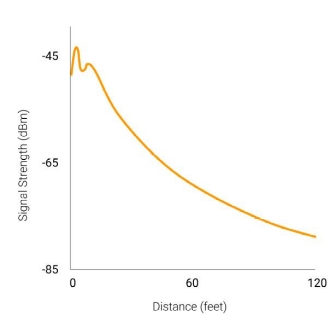
\includegraphics{images/rssi-vs-dist.jpeg}
  \caption{The decay of signal strength (RSSI) with respect to distance.}
  \label{figure:collection:rssivsdist}
\end{marginfigure}
\marginnote[0.5em]{\fontsize{7}{7}\textit{Source: Wi-Fi Location-Based Services, Cisco }}

All these factors vary widely in real world conditions at each location depending on where and how the sensors are installed.
They also vary widely over time due to changes in the context and vary across different directions at each location as well.
This makes it extremely difficult to model the distance between mobile device and the access point as a function of the received signal strength.
The equation \ref{equation:rssi:hard} can be approximated and simplified as,

\begin{equation}
  R = (-10 \times \log_{10}{d}) + A
  \label{equation:rssi:simple}
\end{equation}

Where \(R\) is the reported signal strength and \(A\) is the signal strength at 1 meter.
Though equation \ref{equation:rssi:simple} can help us to infer the distance of the mobile device roughly, the location wise uncertainty of this method makes it lose the meaning when compared across locations.

From the above we can conclude that it is almost impossible to delineate the field of measurement precisely and accurately by simple methods using the information present in the probe requests.
This leads to uncertainty in the data collected which needs to be resolved with explicit assumptions or specific methods to reduce the resulting noise.
We require a method to isolate this noise from data generated by devices within the field of measurement.
This methods needs to be independent of the micro site configuration, temporal changes in the context.

%------------------------------------------------------------------------------%
\subsection{Probe request frequency}
%------------------------------------------------------------------------------%
The second uncertainty we face is the frequency at which mobile devices generated the probe requests which varies wildly.
The number of probe requests generated from a mobile device depends on,

\begin{enumerate}
  \setlength{\itemindent}{2em}
  \itemsep-0.5em
  \item Manufacturer of the device. E.g. Samsung vs Apple
  \item Version of the software running on the device. E.g iOS 7 vs iOS 8
  \item State of the device. E.g. If it is already connected to internet? Has the location services been switched off?
  \item The number of access points already known to the device.
\end{enumerate}

Studies done by \citet{freud2015}\cite{freud2015} has shown that the number of probe requests generated by a mobile device vary widely across manufacturers such as Samsung, Apple and LG, across different state the devices are in such as charging, screen being on, Airplane mode being on etc and depends heavily on the number of access points known to the device.
It is also seen from our initial experiments that these probe requests are generated in short bursts rather than being generated at regular intervals.
This makes predicting a base factor for calculating a number of mobile devices based on the number of probe requests received much more complex.
The variety of device models available and the pace of change in software that run these models further complicates this.
Though we can simply aggregate these probe requests based on the unique information on them, in absence of such information it becomes extremely critical.
We to consider this uncertainty in detail while making any simple assumptions on the relationship between number of probe requests and the number of mobile devices that generated them.

%------------------------------------------------------------------------------%
\subsection{MAC address randomisation}
%------------------------------------------------------------------------------%
Randomisation of MAC address is one of the recent uncertainty introduced in the data.
As we saw in section \ref{wifi-as-source-of-data} MAC address is the unique identifier for each mobile device and we aggregate the footfall numbers based on this.
Since the probe requests are transmitted unencrypted and can be received by any access point, this is one of the biggest leak of personal data which occurs in the Wi-Fi based communications.
Modern mobile devices solve this problem by using a randomised MAC address for the probe requests which can result in large over estimation of number of mobile devices in the vicinity.

\begin{marginfigure}
  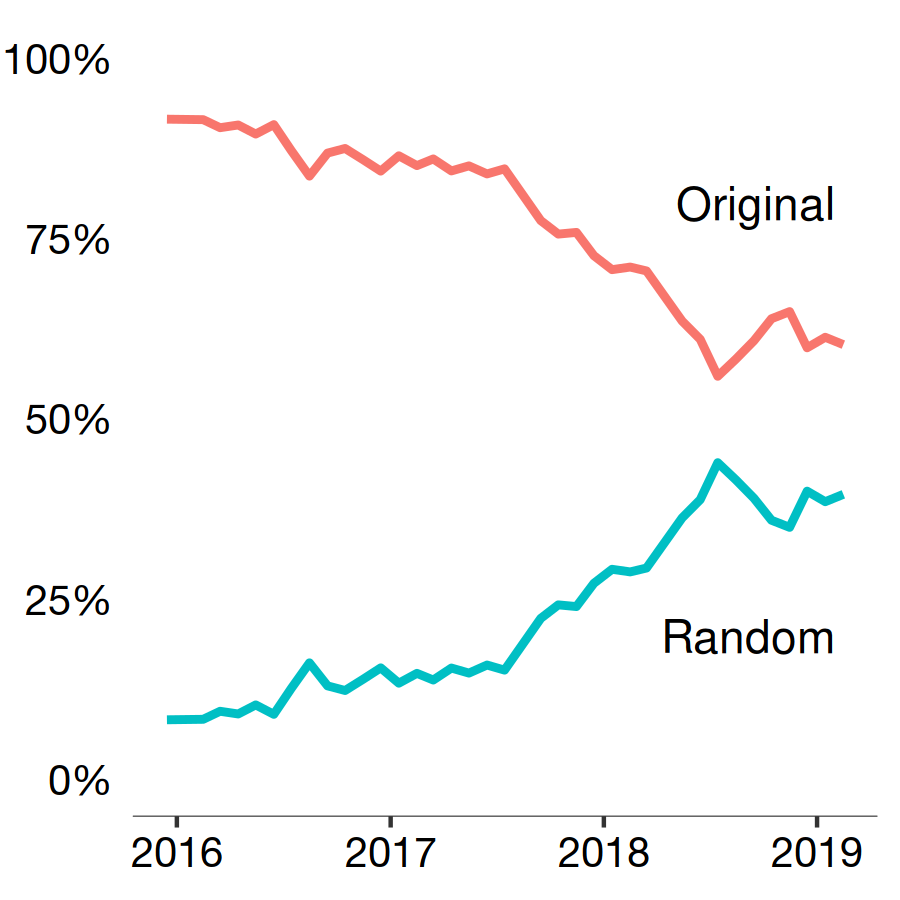
\includegraphics{images/mac-randomisation.png}
  \caption{Increase in the share of randomised MAC addresses compared to non-randomised original ones over the years.}
  \label{figure:collection:macrandom}
\end{marginfigure}
\marginnote{\fontsize{7}{7}\textit{From data collected at Regent Street, Cambridge.}}

The method of randomisation and the frequency varies widely between device manufacturers and also changes as new versions of the software are released.
This seriously affects the usefulness of the data long term where methods designed to overcome this randomisation can be rendered inefficient in the future.
Figure \ref{figure:collection:macrandom} shows the increase in the share of randomised MAC addresses since 2015.
We can observe that in addition to the overall upward trend there are bursts of increase around late 2016 and 2017 which coincides with the release of new mobile operating systems.
This makes it necessary for devising a method to overcome MAC randomisation problem to be able to uniquely fingerprint devices so that they can be aggregated together.
As we saw in our literature review, this is also one of the major opportunities in research on human mobility using Wi-Fi data.

%------------------------------------------------------------------------------%
\subsection{Mobile Device Ownership}
%------------------------------------------------------------------------------%
One of the major external bias in all the datasets collected from mobile devices is the overall volume and nature of the ownership of these devices.
The ownership of mobile devices, specifically Wi-Fi enabled ones, have been on the rise since 2005.
Though mobile ownership has reached unprecedented level in recent years, there is still an underlying increasing trend present in the ownership of these devices which manifests itself in the collected data.
Moreover the mobile ownership varies widely between demography of age and geography as well. 
Figure \ref{figure:collection:ownership} shows the mobile ownership across age groups in UK from 2012 to 2018.
We can observe that the older age groups are under-represented in our data.
This needs to be taken into consideration while using this data for extrapolating demographic conclusions out of it.
In addition to this, the overall upward trend needs to be adjusted assuming 1\% increase monthly and 0.2\% weekly when using this data across long periods of time.

\begin{marginfigure}
  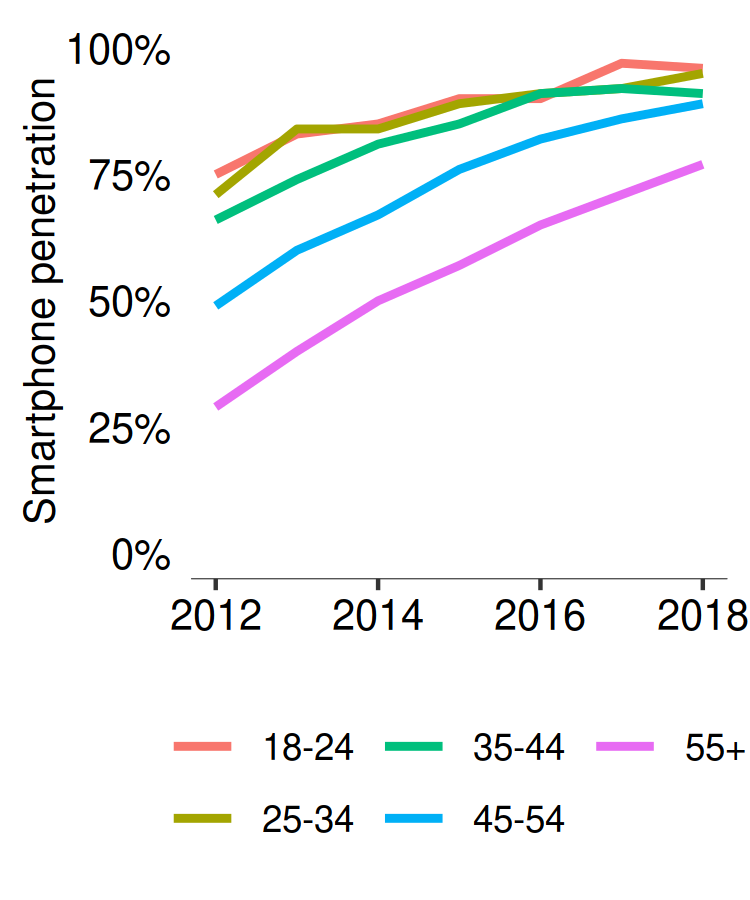
\includegraphics{images/mobile-ownership.png}
  \caption{Smartphone penetration by age group in United Kingdom (2012-18)}
  \label{figure:collection:ownership}
\end{marginfigure}
\marginnote{\fontsize{7}{7}\textit{Source: UK edition, Deloitte Global Mobile Consumer Survey, }}



%------------------------------------------------------------------------------%
\subsection{Missing Data}
%------------------------------------------------------------------------------%
Being collected by distributed set of sensors located in busy real-world scenarios, the data has a large number of gaps as well.
These gaps are caused by various reasons such as, failure of the sensor hardware and software, failure in internet connectivity to send the data back, External factors such as store closures which can cause power loss, regular disruptions such as software update and maintenance and finally other factors such as unauthorised tampering and unplugging of the sensor.
This is leads to a dataset which contains several small and medium sized gaps as shown in Figure \ref{figure:toolkit:veracity:gaps}.
More over, the Smart Street Sensor project is implemented and managed with commercial motive, the sensors are installed and uninstalled at locations as retail partners join and leave the project.
This leads to an uneven availability of data across locations over longer time periods which creates challenges while aggregating data across locations.
We need to implement a methodology to fill in these gaps which considers the periodic patterns in the data.
We also need to devise a measure for aggregating the counts across locations which removes the bias introduced by long term gaps in data.

%------------------------------------------------------------------------------%
\subsection{MAC address collisions}
%------------------------------------------------------------------------------%
Finally, from the initial analysis we have observed that there are few instances of collisions occurring in the hashed MAC addresses.
This has been observed as unique hashed MAC addresses appear at different locations within a short period of time which cannot be explained by the physical travel by the user between these locations.
These collisions are caused by the limitation of the hashing algorithm used and exist only in very large amounts of data.
It is important to note that this collision are specific to non-randomised MAC addresses as we don't expect any consistency within the randomised ones.
Even though this is an inevitable side effect of the hashing process, the probability of such occurrence is very low and is calculated as \(2^{-n}\), where \(n\) is the number of bits in the output of the hashing algorithm.
The total number of estimated collisions between \(m\) unique values is given by, \(2^{-n} \times {m \choose 2}\)\cite{estcollision}.
This translates to around 100 collisions across a million unique devices with a 32 bit algorithm and 2 collisions across 10 Billion devices when using a 64 bit algorithm. 
Though these collisions might cause issues in granular mobility models, for long term and broad studies where we don't track individual devices, they can be safely ignored.
